\documentclass{article}	
\usepackage[utf8]{inputenc} 		
\usepackage{amsmath} 

\usepackage{verbatim}
\usepackage{fancyhdr}
\usepackage{lastpage}
\usepackage{lineno}
\usepackage{lmodern}
\usepackage[T1]{fontenc}
\usepackage[utf8]{inputenc}
\usepackage{microtype}
\usepackage{systeme}
\usepackage{amsmath,amssymb,amsthm,mathrsfs,latexsym,tikz,url}
\usepackage{epigraph,graphicx}
\usepackage{titlesec} %For formatting sections
\usepackage{listings}
\usepackage{listingsutf8}
\usepackage{color}
\usepackage{todonotes}
\usepackage{caption}
\usepackage{float}
\usepackage{cite}
\usepackage[font=small,labelfont=bf]{caption}
\presetkeys%
    {todonotes}%
    {inline,backgroundcolor=yellow}{}

\graphicspath{ {./}{./figures/} {images/}}
\DeclareGraphicsExtensions{.png,.pdf}

\definecolor{dkgreen}{rgb}{0,0.6,0}
\definecolor{gray}{rgb}{0.5,0.5,0.5}
\definecolor{mauve}{rgb}{0.58,0,0.82}

\lstset{frame=tb,
  language=Java,
  aboveskip=3mm,
  belowskip=3mm,
  showstringspaces=false,
  columns=flexible,
  basicstyle={\small\ttfamily},
  numbers=none,
  numberstyle=\tiny\color{gray},
  keywordstyle=\color{blue},
  commentstyle=\color{dkgreen},
  stringstyle=\color{mauve},
  breaklines=true,
  breakatwhitespace=true,
  tabsize=3
}


\setlength{\parindent}{0.0cm}
\setlength{\parskip}{0.1cm}

% \renewcommand{\familydefault}{ptm} %New Century Schoolbook
%pnc =  New Century Schoolbook
%ppl = palatino
%ptm = times new roman



% \titleformat{<command>}[<shape>]{<format>}{<label>}{<sep>}{<before-code>}[<after-code>]

\titleformat{\section}{\normalfont\scshape}{\thesection.}{1em}{}
% \titlespacing{\section}{0pc}{1.5ex plus .1ex minus .2ex}{0pc}
% %
% \titleformat{\subsection}[runin]{\normalfont\bfseries}{\thesubsection}{1em}{}
\titleformat{\subsection}{\normalfont\bfseries}{\thesubsection}{1em}{}
% \titlespacing{\subsection}{0pc}{1.5ex plus .1ex minus .2ex}{1pc}


%%%%%%%%%%%%%%%%%%%%%%%%%%%%%%%%%%%%%%%%%%%%%%%%%%%%%%%%%%%%%%%%%%%%%%%%%%%%%%%%%%%








% See http://texblog.org/2007/11/07/headerfooter-in-latex-with-fancyhdr/
\fancyhead[R]{Jan Alexandersson, \thepage/\pageref{LastPage}}





\begin{document}


\title{Assignment 1 Deep Learning}
\author{Jan Alexandersson}
\maketitle 


\section{Check gradient}

\begin{lstlisting}
def ComputeGradients(X,Y,W,b, lamb):	
	P = EvaluateClassifier(X, W, b)
	g = -(Y-P)
	
	grad_W = np.matmul(g, X.T) / X.shape[1] + 2*lamb*W
	grad_b = np.matmul(g, np.ones((X.shape[1], 1))) / X.shape[1]
	
	return grad_W, grad_b
\end{lstlisting}


I checked the relative error between numerically computed gradient and analytically computed gradient 

\begin{equation}
 \varepsilon = \max (|g_a - g_n| ./ \max(\text{eps} , |g_a + g_n|)),
\end{equation}

where $\text{eps} = 1e-6$, and we can see the result in the table below. 

\begin{center}
\begin{tabular}{ |c|c|c|c| } 
\hline
Batch size = & 10 & 100 \\
\hline
$\varepsilon_b$ = & 4.1887087217846966e-07 & 6.364790025496572e-07  \\
\hline
$\varepsilon_W$ = & 1.886843874610762e-07 &  3.415967157102575e-07 \\ 
\hline
\end{tabular}
\end{center}

This was when using \textbf{lambda = 0}. Since all relative errors are small we conclude that our implementeation of the 
analytical gradient is correct. 

\section{Results}

We used the settings \textbf{n\_epochs = 40, n\_batch = 100} for all the runs and we got, for different values of 
\textbf{lambda} and \textbf{eta}, the result below. 

\begin{center}
\begin{tabular}{ |c|c|c| } 
\hline
Parameters  &  Training accuracy & Test accuracy  \\
\hline
 Eta $= 0.1$, lambda $= 0$ & 0.4487 & 0.2898 \\
\hline
Eta $= 0.001$, lambda $= 0$  & 0.4576 &  0.3907 \\ 
\hline
Eta $= 0.001$, lambda $= 0.1$   & 0.4457 &  0.3904  \\ 
\hline
Eta $= 0.001$, lambda $= 1$  & 0.4017  &  0.3775  \\ 
\hline 
\end{tabular}
\end{center}

We can also plot the cost functions and the images representing the W matrix. These plots are presented below. 

\begin{figure}[H]
\centering
  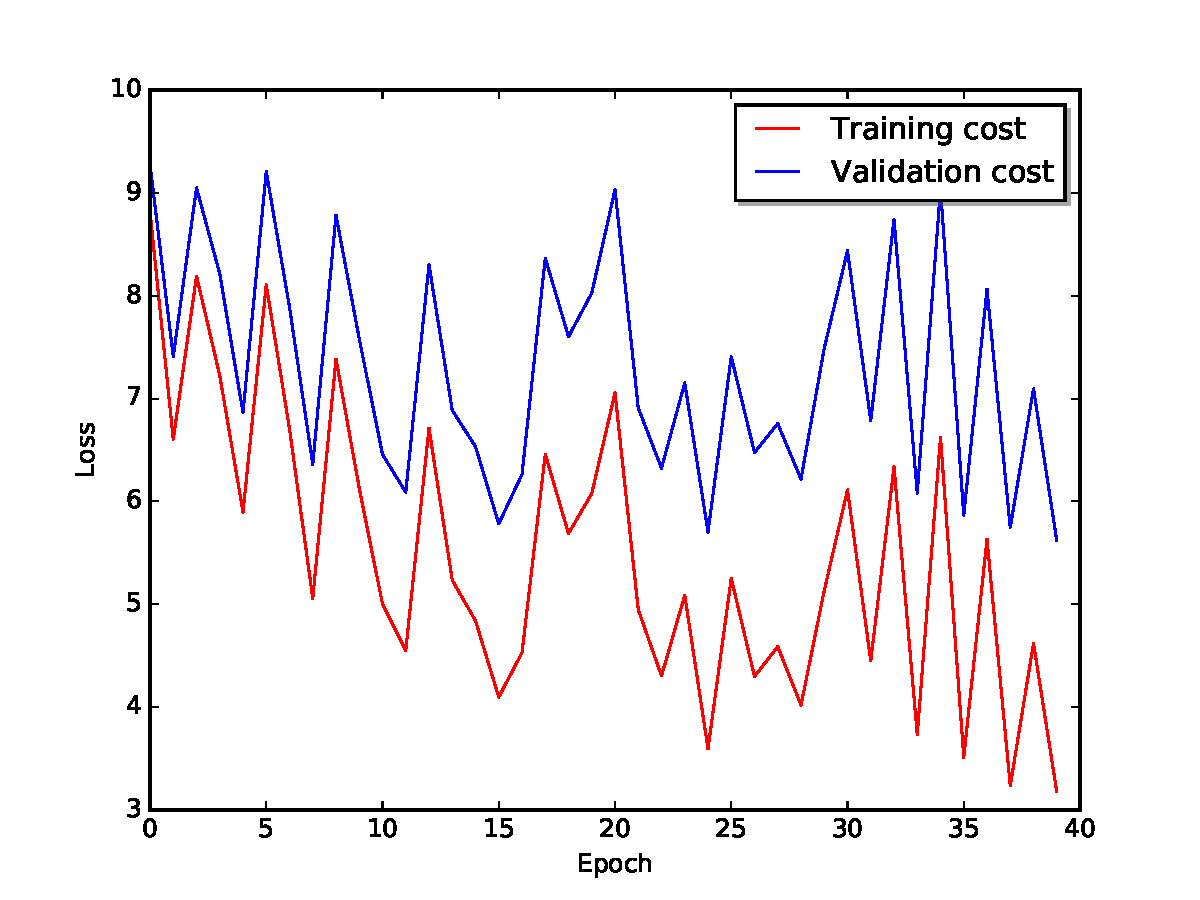
\includegraphics[width = 12cm]{../Result_pics/firstCost2.pdf}
\caption{Cost function using \textbf{lambda = 0, n\_epochs = 40, n\_batch = 100, eta = 0.1}. }
\label{fig:firstCost}
\end{figure}

\begin{figure}[H]
\centering
  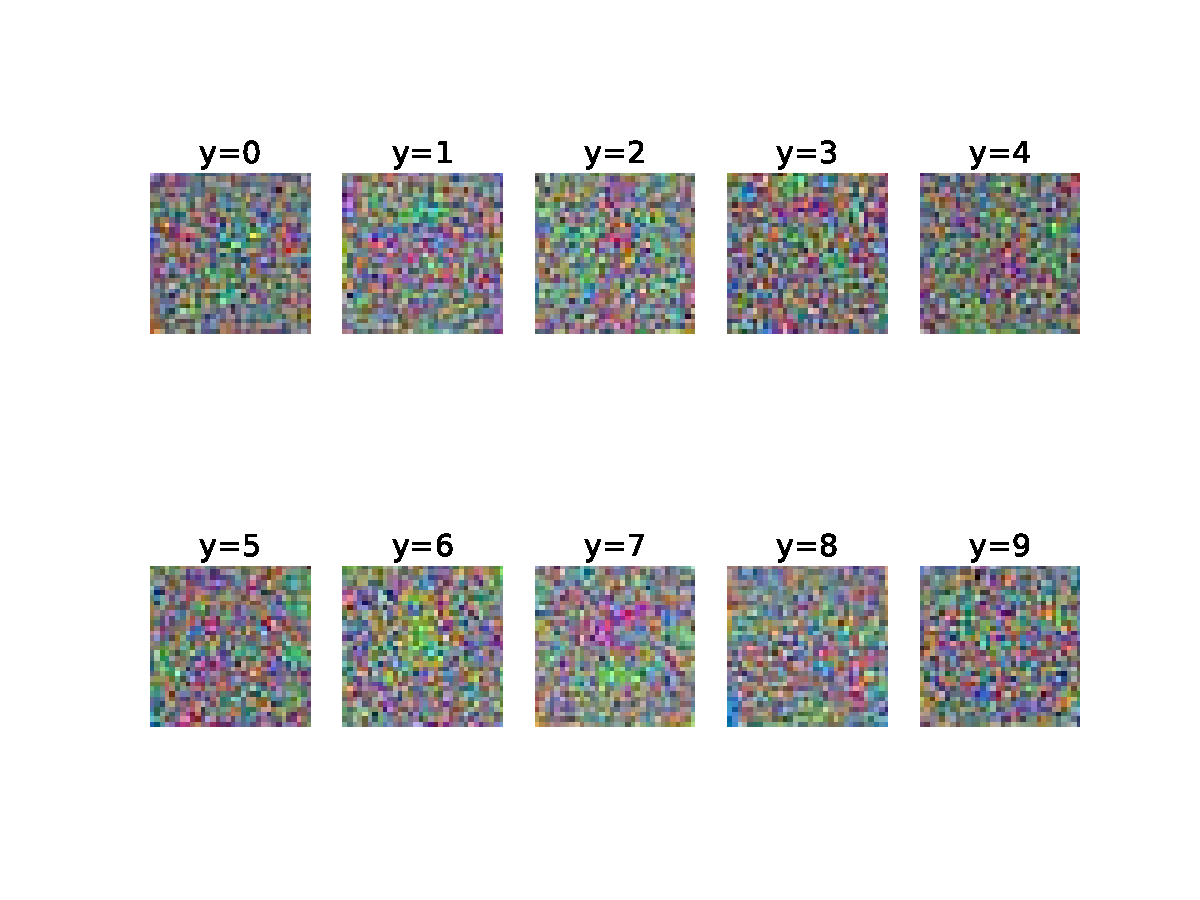
\includegraphics[width = 12cm]{../Result_pics/firstW2.pdf}
\caption{Images representing the W matrix using settings \textbf{lambda = 0, n\_epochs = 40, n\_batch = 100, eta = 0.1}.}
\label{fig:firstW}
\end{figure}


\begin{figure}[H]
\centering
  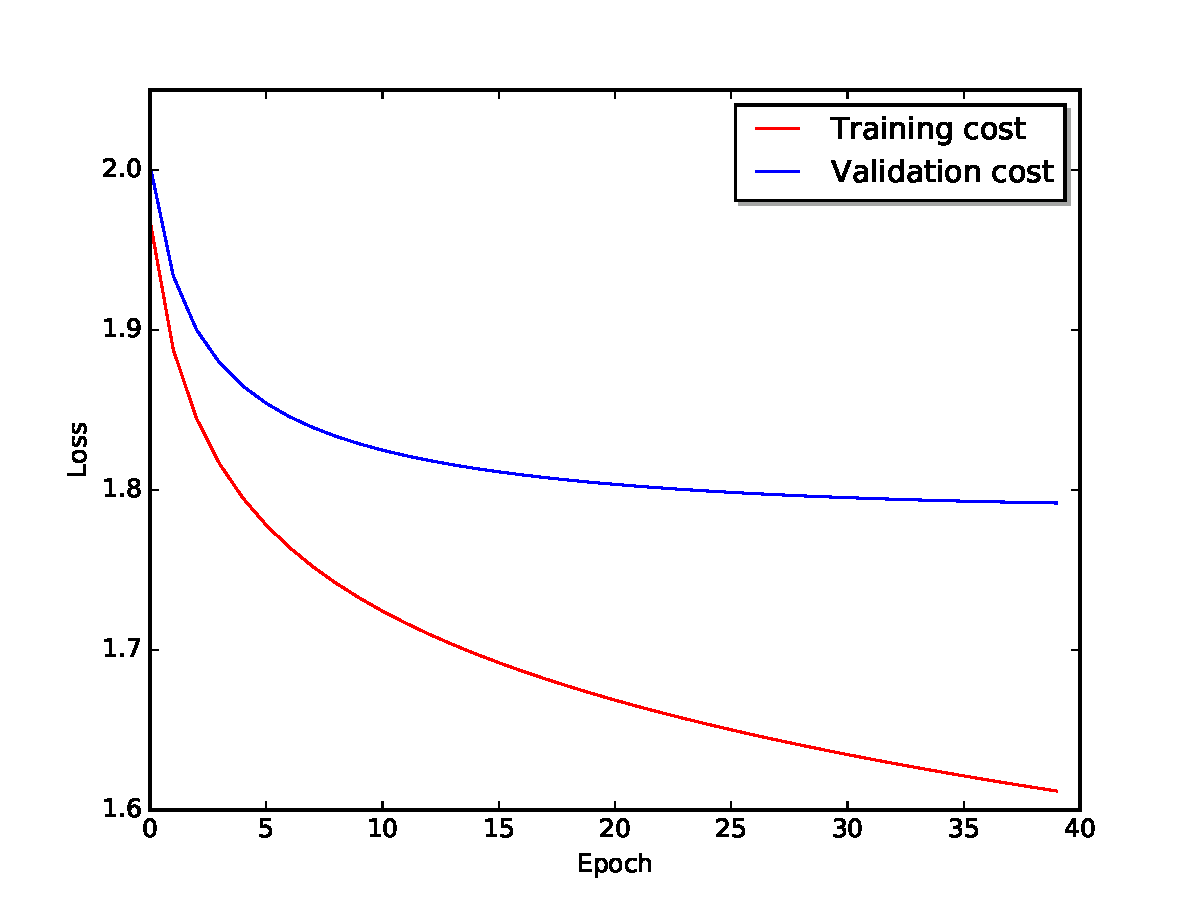
\includegraphics[width = 12cm]{../Result_pics/secondCost2.pdf}
\caption{Cost function using \textbf{lambda = 0, n\_epochs = 40, n\_batch = 100, eta = 0.001}. }
\label{fig:secondCost}
\end{figure}

\begin{figure}[H]
\centering
  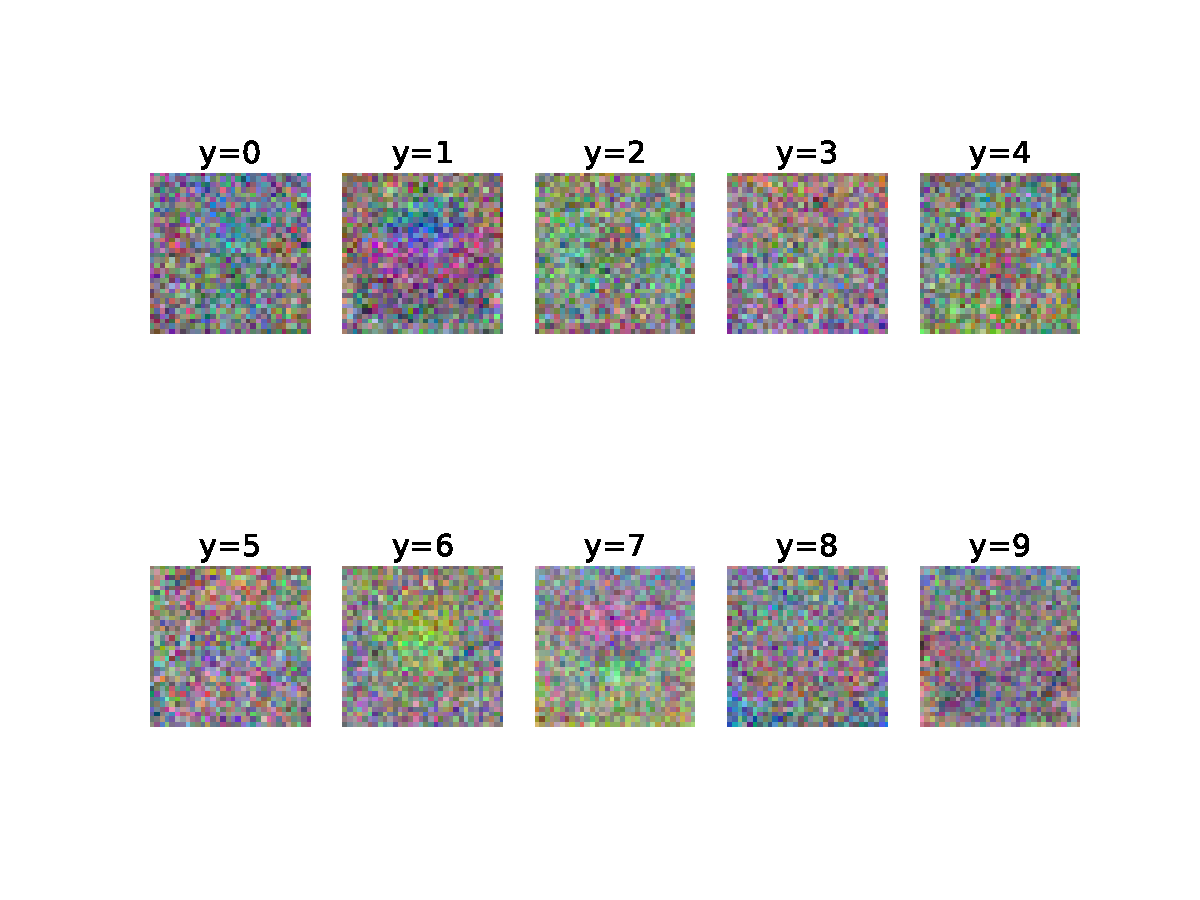
\includegraphics[width = 12cm]{../Result_pics/secondW2.pdf}
\caption{Images representing the W matrix using settings \textbf{lambda = 0, n\_epochs = 40, n\_batch = 100, eta = 0.001}.}
\label{fig:secondW}
\end{figure}


\begin{figure}[H]
\centering
  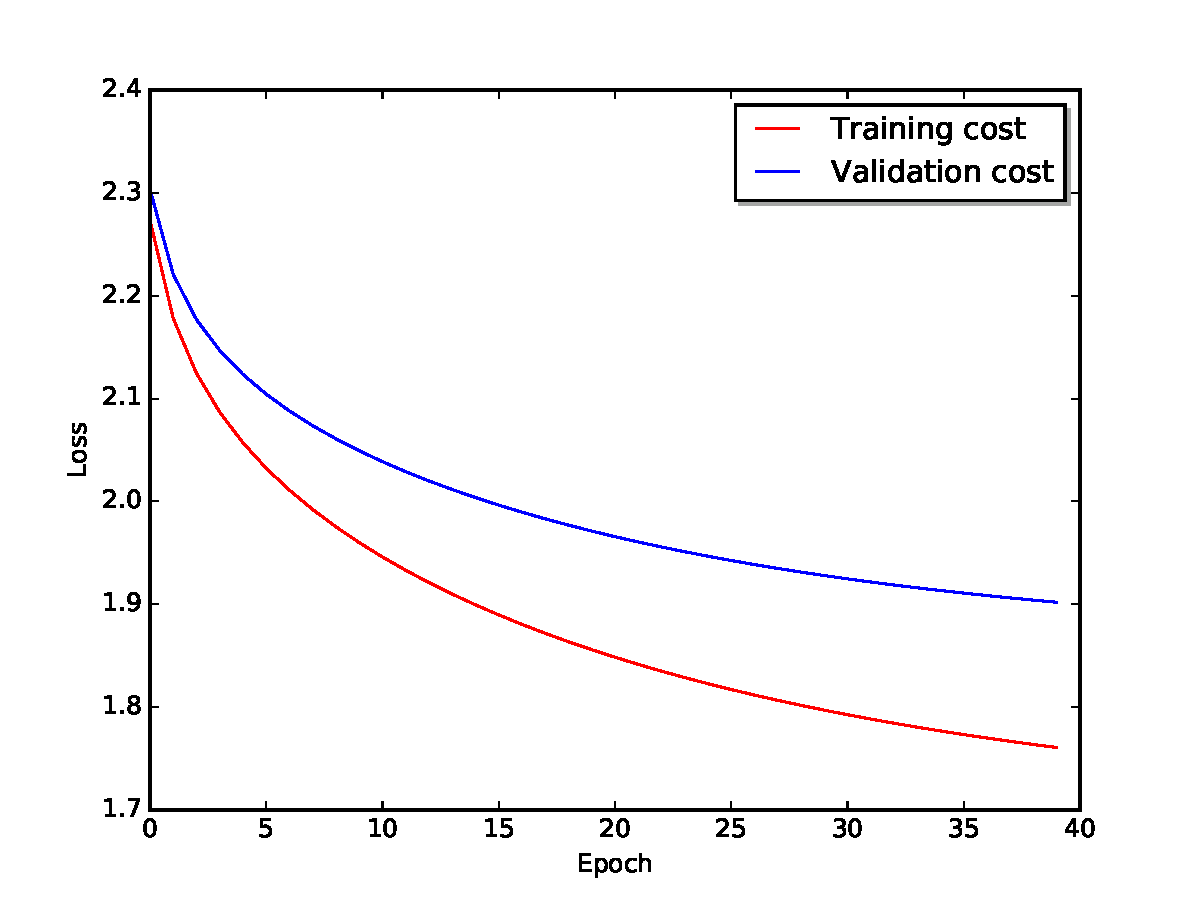
\includegraphics[width = 12cm]{../Result_pics/thirdCost2.pdf}
\caption{Cost function using \textbf{lambda = 0.1, n\_epochs = 40, n\_batch = 100, eta = 0.001}. }
\label{fig:thirdCost}
\end{figure}

\begin{figure}[H]
\centering
  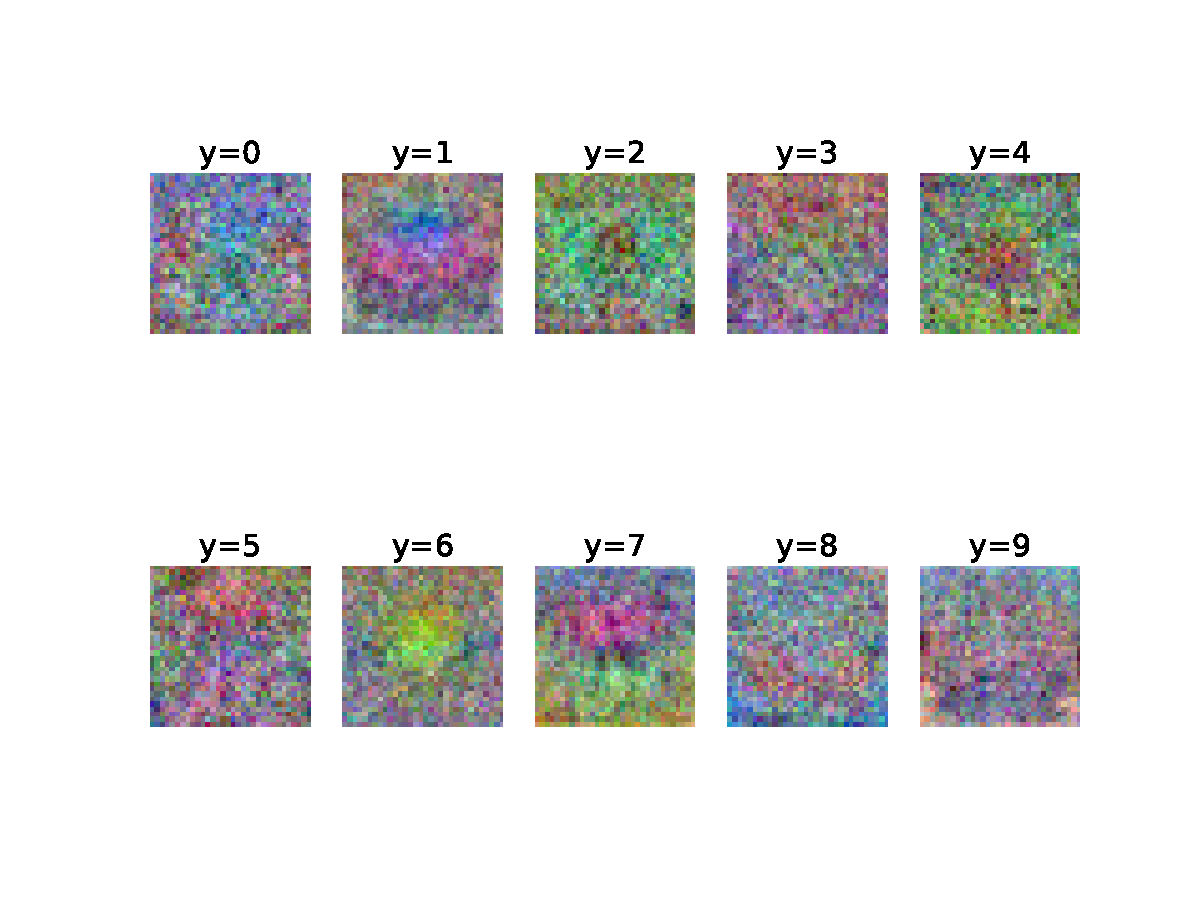
\includegraphics[width = 12cm]{../Result_pics/thirdW2.pdf}
\caption{Images representing the W matrix using settings \textbf{lambda = 0, n\_epochs = 40, n\_batch = 100, eta = 0.001}.}
\label{fig:thirdW}
\end{figure}


\begin{figure}[H]
\centering
  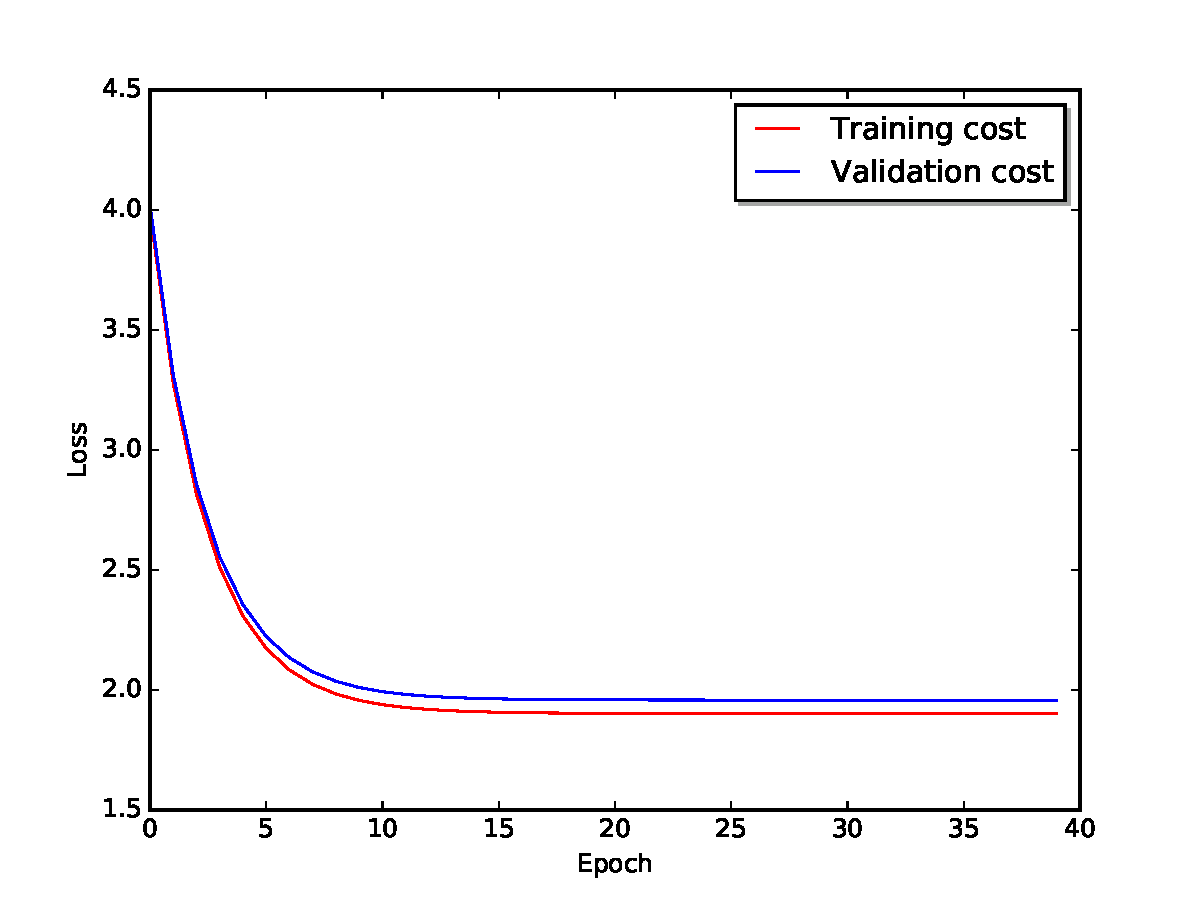
\includegraphics[width = 12cm]{../Result_pics/fourthCost2.pdf}
\caption{Cost function using \textbf{lambda = 1, n\_epochs = 40, n\_batch = 100, eta = 0.001}. }
\label{fig:fourthCost}
\end{figure}

\begin{figure}[H]
\centering
  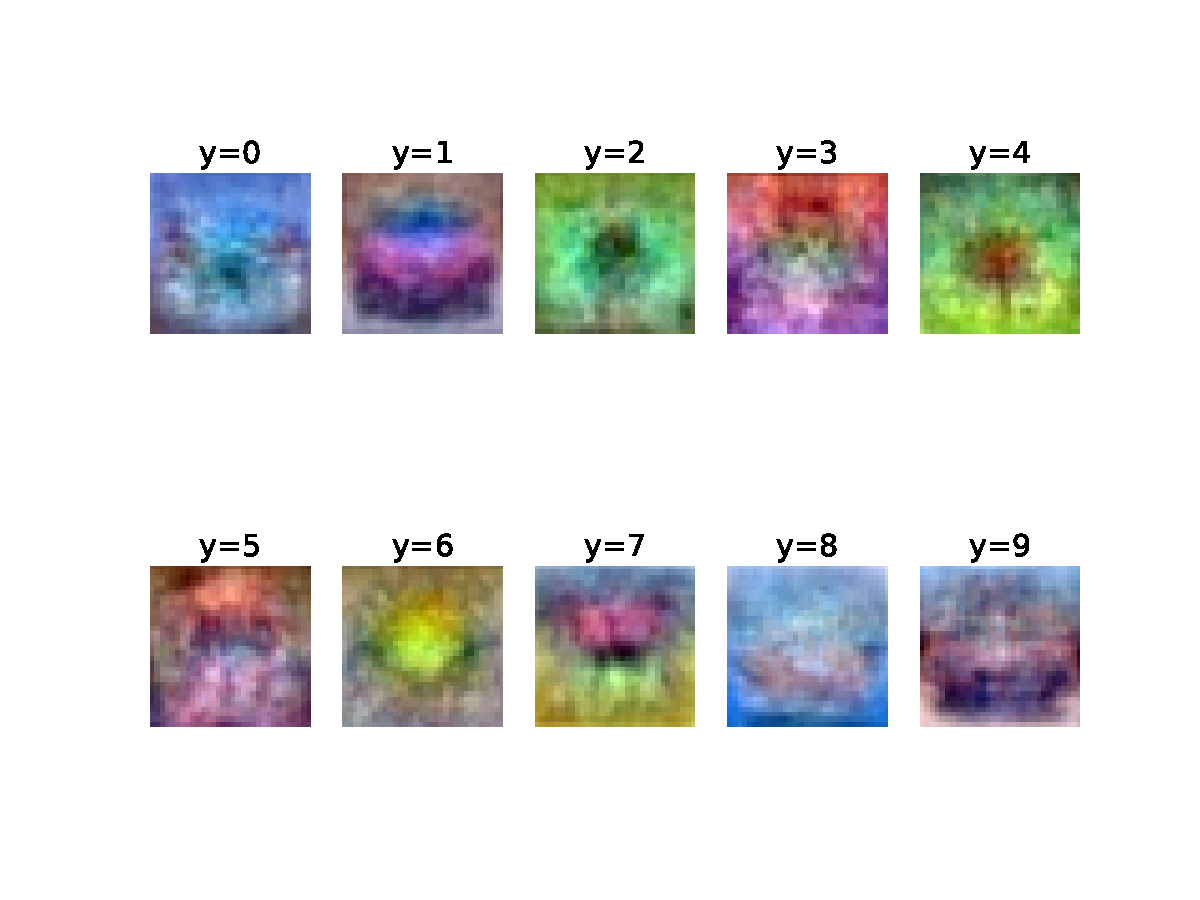
\includegraphics[width = 12cm]{../Result_pics/fourthW2.pdf}
\caption{Images representing the W matrix using settings \textbf{lambda = 1, n\_epochs = 40, n\_batch = 100, eta = 0.001}.}
\label{fig:fourthW}
\end{figure}


When increasing the learning rate the cost function converge faster but is will oscillate be more 
unstable, which we can see in Figure 1. The learning rate is too large and we will jump around the minumum 
and not stay at the minimum when we perform the minibatch gradient decent. 
A lower learning rate will cause the cost function to converge slower but the curve will be more stable and our results 
are more reliable. 

When increasing the regularisation term we get a smoother representation of the W matrix, which we see in Figure 8. 
This is because when increasing the regularisation term we restrict the model and will generalize more, however a too 
large value of the regularisation term will generalize too much and reulst in dropped test accuracy while a too low value 
will cause overfitting. 





\end{document}